%%%%%%%%%%%%%%%%%%%%%%%%%%%%%%%%%%%%%%%%%
% Vertical Line Title Page 
% LaTeX Template
% Version 1.0 (27/12/12)
%
% This template has been downloaded from:
% http://www.LaTeXTemplates.com
%
% Original author:
% Peter Wilson (herries.press@earthlink.net)
%
% License:
% CC BY-NC-SA 3.0 (http://creativecommons.org/licenses/by-nc-sa/3.0/)
% 
% Instructions for using this template:
% This title page compiles as is. If you wish to include this title page in 
% another document, you will need to copy everything before 
% \begin{document} into the preamble of your document. The title page is
% then included using \titleGM within your document.
%
%%%%%%%%%%%%%%%%%%%%%%%%%%%%%%%%%%%%%%%%%
%----------------------------------------------------------------------------------------
%	PACKAGES AND OTHER DOCUMENT CONFIGURATIONS
%----------------------------------------------------------------------------------------
\documentclass{book}
\usepackage{hyperref}
\usepackage{graphicx}
\newcommand*{\plogo}{\fbox{$\mathcal{PL}$}} % Generic publisher logo
%----------------------------------------------------------------------------------------
%	TITLE PAGE
%----------------------------------------------------------------------------------------
\newcommand*{\titleGM}{\begingroup % Create the command for including the title page in the document
\hbox{ % Horizontal box
\hspace*{0.2\textwidth} % Whitespace to the left of the title page
\rule{1pt}{\textheight} % Vertical line
\hspace*{0.05\textwidth} % Whitespace between the vertical line and title page text
\parbox[b]{0.75\textwidth}{ % Paragraph box which restricts text to less than the width of the page
\bigskip \bigskip \bigskip

\includegraphics[width=0.8\textwidth]{desi-960-168}
\bigskip \bigskip \bigskip
{\noindent\Huge\bfseries Documentation}\\[2\baselineskip] % Title
{\large \textrm{\linespread{2} Documentation of all the scripts and functions used to investigate
redshift incompleteness due to galaxies that are not assigned fibres \bigskip \break 
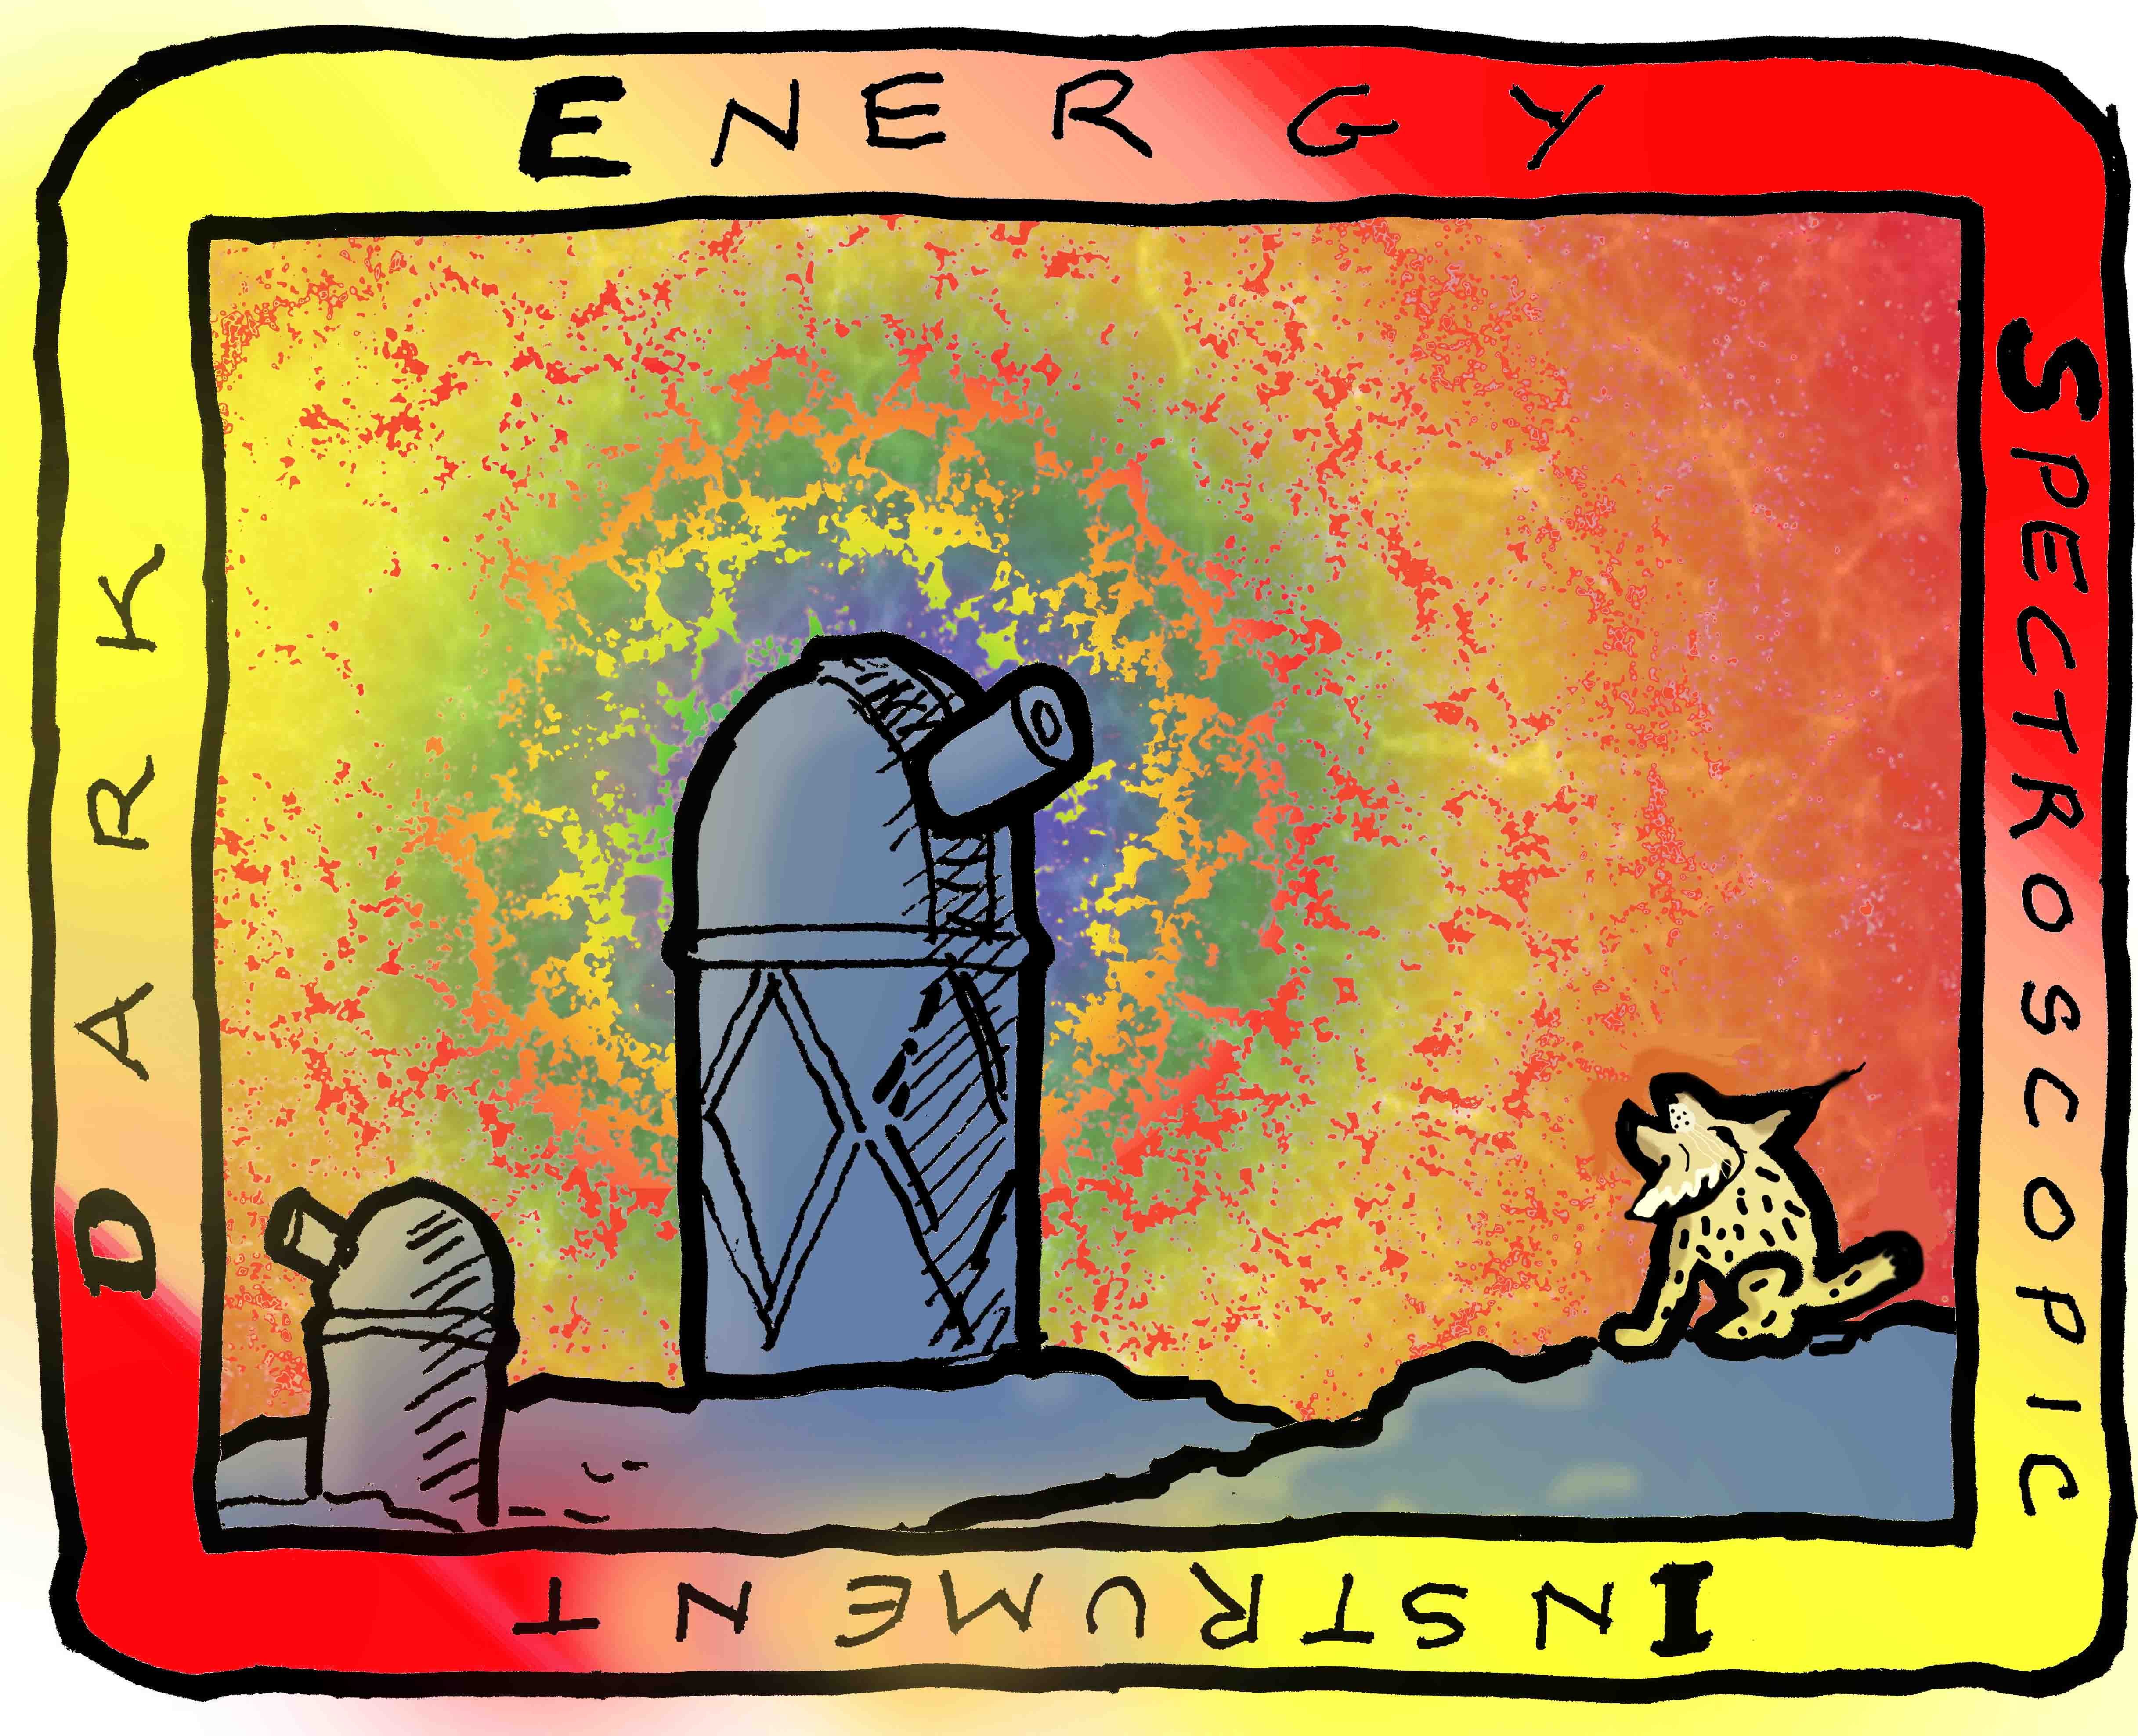
\includegraphics[width=0.5\textwidth]{desisplogo}
\break Part of the \emph{DESI} (Dark Energy Spectroscopic Instrument) project \href{desi.lbl.gov}{desi.lbl.gov} and its \emph{Bright Galaxy Survey} group. }}\\[4\baselineskip] % Tagline or further description
{\Large \textsc{Husni $\! \! \! \! \! \! \! \! \! \! \! \! \! \! \! \! \! \! \! \! \! \! \! \! \! \!  $Almoubayyed }} % Author name
\break\href{mailto:husni@physics.org}{Email: Husni@Physics.org}
\vspace{0.1\textheight} % Whitespace between the title block and the publisher
}}
\endgroup}

%----------------------------------------------------------------------------------------
%	BLANK DOCUMENT
%----------------------------------------------------------------------------------------

\begin{document}

\pagestyle{empty} % Removes page numbers

\titleGM % This command includes the title page

\end{document}